%! TEX root = ../000-main.tex
\section{Kernel design}
\index{kernel!design}

\begin{theorem}[breakable]{Generating valid kernels from other kernels}{}
	Assume $\kappa,\,\kappa' : \mathcal{X} \times \mathcal{X} \to \mathbb{R}$.
	\begin{align*}
		\forall x \in \mathcal{X}, \; \forall a > 0 \in \mathds R, \;
		\kappa(x,x) \geq a \quad \Rightarrow \quad \kappa_a(x,x) \coloneqq a \kappa(x,x) \tag{Mult. by scalar}              \\
		\forall x,x' \in \mathcal{X}, \quad \kappa_n \coloneqq \kappa(x,x') + \kappa'(x, x') \tag{sum}\label{eq:kernel_sum} \\[1em]
		\kappa_1 : \mathcal X_1 \times \mathcal X_1 \to \mathbb R                                                           \\
		\kappa_2 : \mathcal X_2 \times \mathcal X_2 \to \mathbb R ,\quad
		\forall x_1,x_1' \in \mathcal X_1, \quad \forall x_2,x_2' \in \mathcal X_2                                          \\
		\kappa_\oplus
		\left(
		(x_1,x_2), (x_1',x_2')
		\right) \coloneqq \kappa_1(x_1,x_1') + \kappa_2(x_2,x_2') \tag{Direct sum}\label{eq:kernel_direct_sum}
		\\[1em]
		\forall x, x' \in \mathcal X, \quad
		\kappa_\cdot (x, x') \coloneqq \kappa(x,x') \cdot \kappa(x',x) \tag{Product}\label{eq:kernel_product}
		\\[1.5em]
		\kappa_\odot
		: \mathcal X_1 \times \mathcal X_2 \to \mathbb R, \quad
		\forall x_1,x_1' \in \mathcal X_1, \quad \forall x_2,x_2' \in \mathcal X_2                                          \\
		\kappa_\odot
		\left(
		(x_1,x_2), (x_1',x_2')
		\right) \coloneqq \kappa(x_1,x_1') \cdot \kappa(x_2,x_2') \tag{Tensor product}                                      \\[1.5em]
		\text{Given a fn. } g: \mathcal X \to \mathbb R                                                                     \\
		\kappa_g(x, x') \coloneqq g(x) \kappa(x, x') g(x') \tag{Composition}                                                \\[1.5em]
	\end{align*}
	We have a sequence of $\{
		\kappa_n
		\}_{n\in \mathds N}$ with limit $\bar \kappa$ positive:
	$\forall x, x' \lim_{a\to \infty} \kappa_a(x,x') = \bar \kappa(x,x')$.

	$\kappa$ such that $\forall x, x' \in \mathcal X, | \kappa(x,x') | < f$.
	Let $h: x \mapsto \sum_{n=0}^\infty a_n x^n$.
	with $a_n \geq 0$ and radius of convergence $f$.
	Then $\kappa_h(x,x') = h(\kappa(x,x'))$.

	\tcblower
	\begin{align*}
		\kappa : \mathcal X \times \mathcal X \to \mathbb R,                      \\
		\forall n \in \mathds N^+, \forall \{x^1, \ldots, x^n\} \in \mathcal X^n, \\
		c^TKc \geq 0, \forall c \in \mathbb R^n, \quad \text{where } K \coloneqq \begin{pmatrix}
			                                                                         \kappa(x^1, x^1) & \cdots & \kappa(x^1, x^n) \\
			                                                                         \vdots           & \ddots & \vdots           \\
			                                                                         \kappa(x^n, x^1) & \cdots & \kappa(x^n, x^n)
		                                                                         \end{pmatrix}
	\end{align*}

	\begin{proof}\Cref{eq:kernel_sum}:
		\begin{align*}
			K, K'                \\
			K_+ \coloneqq K + K' \\
		\end{align*}
	\end{proof}

	\begin{proof}\Cref{eq:kernel_direct_sum}
		\begin{align*}
			K_1, K_2 \\
			K_\oplus\left(
			(x_1,x_2), (x_1',x_2')
			\right) \coloneqq K_1(x_1,x_1') + K_2(x_2,x_2')
		\end{align*}
	\end{proof}

	\begin{proof}\Cref{eq:kernel_product}
		\begin{align*}
			K, K'                             \\
			K_\cdot \coloneqq K_1 \otimes K_2 \\
		\end{align*}
		(Hadamand product)

		We know that if a matrix $A$ is PSD, then there exists a matrix
		$M$ such that $A = M^TM$.
		\begin{align*}
			\mathlarger{\sum_i} \sum_j
			c_i c_j (K_\cdot)_{ij} & =
			\mathlarger{\sum_i} \sum_j
			c_i c_j \left[
				(K_1)_{ij} \cdot (K_2)_{ij}
			\right]                                                                                    \\
			                       & = \mathlarger{\sum_i} \sum_j
			c_i c_j \left[
				\left(
				\sum_l M_{il} \cdot M_{lj}
				\right) (K_2)_{ij}
			\right]                                                                                    \\
			                       & = \mathlarger{\mathlarger{\sum_l}}
			\left[
				\mathlarger{\sum_i} \sum_j c_i c_j M_{il} M_{lj} (K_2)_{ij}
			\right]                                                                                    \\
			                       & = \sum_l z_l^T K_2 z_l \geq 0                                     \\
			                       &                                    & z_l \coloneqq \begin{pmatrix}
				                                                                            c_1 M_{1l} \\
				                                                                            \vdots     \\
				                                                                            c_n M_{nl}
			                                                                            \end{pmatrix}
		\end{align*}
	\end{proof}

	%   \begin{proof} Limit
	%     \begin{align*}
	%       \forall n \in \mathds N , \{\kappa_n\} \\
	%       \{\kappa_n\}  \to \kappa \\
	%       \kappa_n (x, x') \xrightarrow_{n\to\infty} \kappa(x, x') \forall x, x' \in \mathcal X \\[2em]
	%       c^T\left(
	%       \lim_{n\to\infty} \kappa_n(x, x')
	%       \right) c =
	%       \lim_{n\to\infty} c^T\left(
	%       \kappa_n(x, x')
	%       \right) c
	%     \end{align*}
	%   \end{proof}

\end{theorem}

\begin{example}{}{}
	Prove that $\kappa_{\text{poly}}(x,x') = \left(1 + x^Tx'\right)^d$ is a kernel.
	\begin{align*}
		\text{Define } p(z) = (z + c)^d \\
	\end{align*}
\end{example}

\pagebreak
\subsection{Kernel from distances}
\index{kernel!from distances}

It is natural to create similarity measures from (metric) distances.

\begin{question}{
		How could we create (design) kernels as PSD similarities from distances?
	}
	{}

	What properties are needed for a distance $d$ and an inversion function $g$
	such that $g(d(x,x'))$ is a kernel?
\end{question}

\begin{note}
	Gaussian RBF kernel: $\kappa_{GRBF}(x,x') = \exp\left(-\frac{\lVert x,x' \rVert^2}{2\sigma^2}\right)$
	comes from a distance. (In this case, the distance is the Euclidean distance)
\end{note}

\begin{definition}{Conditionally Negative Semi-Definite (CNSD)}{}
\index{Conditionally Negative Semi-Definite}
\index{CNSD}

	A kernel fn $K: \mathcal \chi \times \mathcal \chi \to \mathbb R$ is CNSD if
	\begin{enumerate}
		\item it is symmetric
		\item $\forall n \in \mathds N^+, \forall \{x^1, \ldots, x^n\} \in \mathcal \chi^n, c^TKc \leq 0$ subject to $c \in \mathds R^n$. $K_{ij} = \kappa(x^i, x^j)$
		      % $\sum_{i=1}^n c_i = 0$
	\end{enumerate}
\end{definition}

\begin{prop}{}{}
	$d(x, x') = \lVert x - x' \rVert^2, \forall x,x' \in \mathds R^d$
	is a CNSD kernel.
\end{prop}

\begin{theorem}{}{}
	Let $\kappa : \chi \times \chi \to \mathbb R$ be a symmetric
	function. Then:
	\begin{align*}
		\kappa\text{ is CNSD } & \iff
		\exp\left(-\gamma \kappa \right),\, \forall \gamma > 0\text{ is PSD}
	\end{align*}

	$\gamma$ is a hyperparameter.
\end{theorem}

We have seen so far that kernel functions are inner products in
some functional space.

\begin{theorem}{Kernel trick for distances}{}
	Let $\kappa : \chi \times \chi \to \mathbb R$ be a CNSD kernel
	such that $\forall x \in \chi,\, x = x' \iff \kappa(x,\,x') = 0$.

	Then, there exists a Hilbert space $\mathcal H$ and a mapping
	$\phi : \chi \to \mathcal H$ such that:
	\begin{equation*}
		\kappa(x, x') = \lVert \phi(x),\, \phi(x') \rVert^2
	\end{equation*}
	Therefore, $\sqrt{\kappa}$ is a metric (Euclidean) distance.
\end{theorem}

\begin{recap}{}{}
	We now have to ways of introducing kernel functions:
	\begin{itemize}
		\item Find a PSD similarity to replace the inner product in the
		      original data space $\chi$.
		\item Find a CNSD kernel to replace the Euclidean distance to
		      replace distances in $\chi$.
	\end{itemize}
\end{recap}

\begin{theorem}{}{}
	Let $\kappa' : \chi \times \chi \to \mathbb R$ be defined
	for an arbitrary $x_0 \in \chi$ as:
	\begin{align*}
		\kappa'(x, x') = \kappa(x, x_0) + \kappa(x_0, x') - \kappa(x, x')
		- \kappa(x_0, x_0) \\[1.5em]
		\boxed{
			\kappa\text{ is CNSD }\iff \kappa'\text{ is PST}
		}
	\end{align*}
\end{theorem}

\subsection{Kernels for sequences}\index{kernel!for sequences}

\begin{marker}
	Sequence and Stream can be taken as synonyms.

	(The main difference is that a stream is continuous,
	while sequences don't have to be)
\end{marker}

\begin{definition}{Alphabet $\Sigma$}{} is a collection of $n$
	different symbols

	\tcblower

	\begin{align*}
		\Sigma & = \{G, A, T, C\}     \\
		\Sigma & = \{0, 1\}           \\
		\Sigma & = \{a, b, \ldots z\}
	\end{align*}
\end{definition}

\begin{question}{How to create good similarity measure between pieces of text?}{}
\end{question}

\begin{align*}
	\Sigma^n                          & = \text{Set of word of length } n       \\
	\Sigma^* = \bigcup_{n>0} \sigma^n & = \text{Set of all words of any length}
\end{align*}

\begin{enumerate}
	\item Chose an integer $p \in \mathds N^+$ (hyperparameter)
	\item Define $\phi^p_\mu(s) = \left| \left\{
		      (v_1, v_2) \mid d = v_1 \mu v_2
		      \right\} \right|$
	\item Define $\kappa_p(s, s') = \phi(s)^T \phi(s')$
	      $= \sum_{\mu \in \Sigma^p} \phi^p_\mu(s) \phi^p_\mu(s')$
\end{enumerate}

\begin{note}\index{spectral kernel}
	We call this Spectral kernel
\end{note}

This is linear in the length of the largest sequence.

This family can be extended usefully in many ways:
\begin{itemize}
	\item Allowing gaps in the common substrings ($\mu$).
	\item Find all common subsequences of all lengths up to length $p$.
	\item Adding weights to the terms (in the inner product) such that
	      we penalize the
\end{itemize}

\subsection{Kernels \emph{from} graphs}\index{kernel!from graphs}

\begin{marker}
	FROM is different that FOR
\end{marker}

We have a data space $\chi$ and a graph of interactions
between data points $x, x' \in \chi$.

In particular, we have:
\begin{itemize}
	\item A training set $D_n = \{x^1,\, \ldots,\, x^n\}$
	\item A graph $G = (V, E)$ where $|V| = n$ and each point $x^i \in V$
	      is associated with a node $v^i \in V$. It is
	      \emph{undirected} and \emph{labelled}.
	      Each edge has a label $l(i,\,j)$ which we call
	      \emph{base similarity}.
	      We encode it as a matrix $B_{ij} = l(i,\,j)$,
	      the matrix must be \emph{symmetric} (since $G$ is undirected).
\end{itemize}

\begin{align*}
	B_{xz} & , x,z \in V                                                        \\
	B_{xz} & = \text{Strength of the connection between nodes } x \text{ and } z
\end{align*}

\begin{figure}[H]
  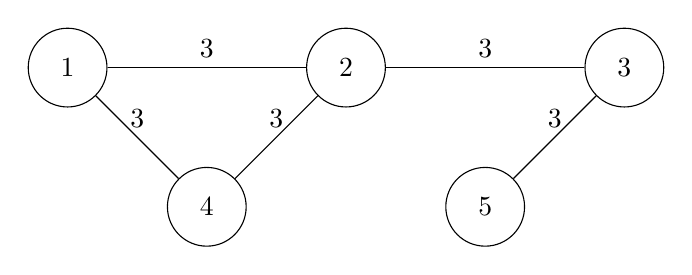
\begin{tikzpicture}[
    node distance=2.5cm,
    vertex/.style={circle, draw, minimum size=1cm},
    ]
    \node[vertex] (a) {$1$};
    \node[vertex, below right of=a] (d) {$4$};
    \node[vertex, above right of=d] (b) {$2$};
    \node[vertex, below right of=b] (e) {$5$};
    \node[vertex, above right of=e] (c) {$3$};

    % edges with weight labels
    \draw (a) -- node[above] {$3$} (b);
    \draw (b) -- node[above] {$3$} (c);
    \draw (a) -- node[above] {$3$} (d);
    \draw (d) -- node[above] {$3$} (b);

    \draw (c) -- node[above] {$3$} (e);

  \end{tikzpicture}
\end{figure}

\begin{align*}
  (B \cdot B)_{i,\,j} &= B^2_{i,\,j} = \mathlarger{\sum_{(i,2,j)}} \prod_{l=1}^2 l(\cdot)
\end{align*}

\begin{theorem}{}{}
  \begin{align*}
    B^0 = I \\
    I + B + B^2 + \ldots \\
    \downarrow \mu \in (0,1) \\
    \mu I + \mu B + \mu^2 B^2 + \ldots \\
    \sum_{b=0}^\infty \frac{\mu^bB^b}{b!} \\
    = \exp(\mu B)
  \end{align*}
\end{theorem}


\begin{definition}{exponential diffusion kernel}{}\index{exponential diffusion kernel}
\begin{equation*}
  \kappa \coloneqq \exp(\mu B) \in \mathds R^{n \times n}
\end{equation*}
\end{definition}
